\documentclass[../thesis]{subfiles}
\begin{document}

\chapter{Background\label{chap:background}}

This chapter describes RISC-V (\cref{chap:bg:sec:riscv}), RVV (\crefrange{chap:bg:rvvstart}{chap:bg:rvvend}), and CHERI (\cref{chap:bg:sec:cheri}) to the detail required to understand the rest of the dissertation.
It summarizes the relevant sections of the RISC-V unprivileged spec\cite{specification-RISCV-vol1-20191213}, the RISC-V ``V'' extension specification v1.0\cite[Sections 1--9, 17]{specification-RVV-v1.0}, the TR-951 CHERI ISAv8 technical report\cite[Chapters 5, 8]{TR-951}, and the TR-949 technical report about C/C++ safety on CHERI\cite[Section 4.4, Appendix C]{TR-949}.
Both vectors and CHERI are described, because this dissertation caters to those who may be familiar with one but not the other.

\section{RISC-V}\label{chap:bg:sec:riscv}
% RISC-V has extensions
RISC-V is an open family of ISAs which defines ``base integer ISAs'' (e.g. all 64-bit RISC-V cores implement the RV64I Base Integer Instruction Set) and extensions (e.g. the ``M'' extension for integer multiplication).
A base instruction set combined with a set of extensions (\todomark{example of a architecture/feature string}) is known as a RISC-V ISA.
Because RISC-V is open, anyone can design, manufacture, and sell chips implementing any RISC-V ISA.

Each RISC-V implementation has a set of constant parameters.
The most common example is \code{XLEN}, the length of an integer register in bits, which is tied to the base integer ISA (e.g. 64-bit ISA implies \code{XLEN=64}).
Other constant parameters include \code{CLEN}, the length of a capability in bits, defined by CHERI relative to \code{XLEN}; and \code{VLEN} and \code{ELEN}, which are used by RVV and entirely implementation-defined.

The extensions of most relevance to this project are the ``V'' vector extension (RVV) and the CHERI extension.
RVV recently became the officially ratified vector extension for RISC-V, which all RISC-V vector processing chips should implement going forward.
The following sections summarize the vector extension, how it accesses memory, and previous implementations in academia.
% \todomark{finish this para}

% RVV is the officially ratified vector extension for RISC-V, and going forward all RISC-V chips with vector processing capabilities should implement it instead of designing their own custom vector extensions.
\pagebreak
\section{A brief history of vector processing}
Many vector implementations (Intel SSE/AVX, Arm's Advanced SIMD and Neon) use fixed-length vectors - e.g. 128-bit vectors which a program interprets as four 32-bit elements.
As the industry's desire for parallelism grew, new implementations had to be designed with longer vectors of more elements.
For example, Intel SSE/SSE2 (both 128-bit) was succeeded by AVX (128 and 256-bit), then AVX2 (entirely 256-bit), then AVX-512 (512-bit).
Programs built for one extension, and hence designed for a specific vector size, could not automatically take advantage of longer vectors.

Scalable vectors address this by not specifying the vector length, and instead calculating it on the fly.
Instead of hardcoding \enquote{this loop iteration uses a single vector of four 32-bit elements}, the program has to ask \enquote{how many 32-bit elements will this iteration use?}.
This gives hardware designers more freedom, letting them select a suitable hardware vector length for their power/timing targets, while guaranteeing consistent execution of programs on arbitrarily-sized vectors.
RVV uses a scalable vector model.

\todomark{better segue into RVV here?}
\section{The RVV vector model}\label{chap:bg:sec:rvv:vector_model}
\emph{Summarizes \cite[Sections 1-6, 17]{specification-RVV-v1.0}}

\figinput[width=0.7\textwidth,pos=h]{1_20Background/figures/fig_RVV_added_state}

RVV defines thirty-two vector registers, each of an implementation-defined constant width \code{VLEN}.
These registers can be interpreted as \emph{vectors} of \emph{elements}.
The program can configure the size of elements, and the implementation defines a maximum width \code{ELEN}.
\cref{fig:RVV_simple_widths} shows a simple example of a 128-bit vector, where the maximum element length is 32-bits.

RVV also adds some state that defines how the vector registers are used (see \cref{fig:RVV_added_state}).
These are stored in RISC-V Control and Status Registers (CSRs), which the program can read.
\code{vtype} (\cref{chap:bg:subsec:vtype}) defines how the vector registers are split into elements.
\code{vstart} and \code{vl} (\cref{chap:bg:subsec:vlvstart}) divides the elements into three disjoint subsets: \emph{prestart}, the \emph{body}, and the \emph{tail}.
Masked accesses (\cref{chap:bg:subsec:rvvmasking}) further divide the \emph{body} into \emph{active} and \emph{inactive} elements.
This section also describes the vector exception model (\cref{chap:bg:subsec:vexceptions}).

\figinput[width=0.7\textwidth,pos=h]{1_20Background/figures/fig_RVV_simple_widths}

%---------------------------------
\subsection{\code{vtype}}\label{chap:bg:subsec:vtype}
\figinput[width=0.7\textwidth,pos=b]{1_20Background/figures/fig_RVV_LMUL_widening}
The \code{vtype} CSR contains two key fields that describe how vector instructions interpret the contents of vector registers.
The first is the Selected Element Width (\code{SEW}), which is self-explanatory.
It can be 8, 16, 32, or 64.
128-bit elements are referenced a few times throughout but haven't been formally specified (see \cite[p10, p32]{specification-RVV-v1.0}).
% Most instructions\footnote{Except where the width is encoded in the instruction, like bytemask loads.} will split vector registers into elements of this width.

The second field is the Vector Register Group Multiplier (\code{LMUL}).
Vector instructions don't just operate over a single register, but over a register \emph{group} as defined by this field.
For example, if \code{LMUL=8} then each instruction would operate over 8 register's worth of elements.
These groups must use aligned register indices, so if \code{LMUL=4} all vector register operands should be multiples of 4 e.g. \code{v0, v4, v8} etc.
In some implementations this may increase throughput, which by itself is beneficial for applications.

However, the true utility of \code{LMUL} lies in widening/narrowing operations (see \cref{fig:RVV_LMUL_widening}).
For example, an 8-by-8-bit multiplication can produce 16-bit results.
Because the element size doubles, the number of vector registers required to hold the same number of elements also doubles.
Doubling \code{LMUL} after such an operation allows subsequent instructions to handle all the results at once.
At the start of such an operation, fractional \code{LMUL} (1/2, 1/4, or 1/8) can be used to avoid subsequent results using too many registers.

\code{vtype} also encodes two flags: mask-agnostic and tail-agnostic.
If these are set, the implementation is \emph{allowed} to overwrite any masked-out or tail elements with all 1s.

Most vector instructions will interpret their operands using \code{vtype}, but this is not always the case.
Some instructions (such as memory accesses) use different Effective Element Widths (\code{EEW}) and Effective LMULs (\code{EMUL}) for their operands.
In the case of memory accesses, the \code{EEW} is encoded in the instruction bits and the \code{EMUL} is calculated to keep the number of elements consistent.
Another example is widening/narrowing operations, which by definition have to interpret the destination registers differently from the sources.

Programs update \code{vtype} through the \code{vsetvl} family of instructions.
These are designed for a ``stripmining'' paradigm, where each iteration of a loop processes some elements until all elements are processed.
\code{vsetvl} instructions take a requested \code{vtype} and the number of remaining elements to process (the Application Vector Length or \code{AVL}), and return the number of elements that will be processed in this iteration.
This value is saved in a register for the program to use, and also saved in the internal \code{vl} CSR.

%---------------------------------
\subsection{\code{vl} and \code{vstart} --- Prestart, body, tail}\label{chap:bg:subsec:vlvstart}
The first CSR is the Vector Length \code{vl}, which holds the number of elements that could be updated from a vector instruction.
The program updates this value through fault-only-first loads (\cref{chap:bg:sec:rvv:fof}) and more commonly \code{vsetvl} instructions.

In the simple case, \code{vl} is equal to the total available elements (see \cref{fig:RVV_vl_full}).
It can also be fewer (see \cref{fig:RVV_vl_short}), in which case vector instructions will not write to elements in the \enquote{tail} (i.e. elements past \code{vl}).
This eliminates the need for a `cleanup loop' common in fixed-length vector programs.

\figinput[width=0.7\textwidth,pos=t]{1_20Background/figures/fig_RVV_vl}

In a similar vein, \code{vstart} specifies \enquote{the index of the first element to be executed by a vector instruction}.
Elements before \code{vstart} are known as the \emph{pre-start} and are not touched by executed instructions.
It is usually only set by the hardware whenever it is interrupted mid-instruction (see \cref{fig:RVV_vstart_trap} and \cref{chap:bg:subsec:vexceptions}) so that the instruction can be re-executed later without corrupting completed values.
Whenever a vector instruction completes, \code{vstart} is reset to zero.

The program \emph{can} set \code{vstart} manually, but it may not always work.
If an implementation couldn't arrive at the value itself, then it is allowed to reject it.
The specification gives an example where a vector implementation never takes interrupts during an arithmetic instruction, so it would never set \code{vstart} during an arithmetic instruction, so it could raise an exception if \code{vstart} was nonzero for an arithmetic instruction.

\figinput[width=0.7\textwidth,pos=t]{1_20Background/figures/fig_RVV_vstart_trap}

\figinput[width=0.8\textwidth,pos=h]{1_20Background/figures/fig_RVV_mask_example}
%---------------------------------
\subsection{Masking --- Active/inactive elements}\label{chap:bg:subsec:rvvmasking}
Most vector instructions allow for per-element \emph{masking} (see \cref{fig:RVV_mask_example}).
When masking is enabled, register \code{v0} acts as the `mask register', where each bit corresponds to an element in the vector\footnote{A single vector register will always have enough bits for all elements. The maximum element count is found when SEW is minimized (8 bits) and LMUL is maximized (8 registers), and is equal to \code{VLEN * LMUL / SEW = VLEN * 8 / 8 = VLEN}.}.
If the mask bit is 0, that element is \emph{active} and will be used as normal.
If the mask bit is 1, that element will be \emph{inactive} and not written to (or depending on the mask-agnostic setting, overwritten with 1s).
When masking is disabled, all elements are \emph{active}.

\pagebreak
%---------------------------------
%---------------------------------
%---------------------------------
\subsection{Exception handling}\label{chap:bg:subsec:vexceptions}
\emph{Summarizes \cite[Section 17]{specification-RVV-v1.0}}

During the execution of a vector instruction, two events can prevent an instruction from fully completing: a synchronous exception in the instruction itself, or an asynchronous interrupt from another part of the system.
Implementations may choose to wait until an instruction fully completes before handling asynchronous interrupts, making it unnecessary to pause the instruction halfway through, but synchronous exceptions cannot be avoided in this way (particularly where page fault exceptions must be handled transparently).

The RVV specification defines two modes for `trapping' these events, which implementations may choose between depending on the context (e.g. the offending instruction), and notes two further modes which may be used in further extensions.
All modes start by saving the PC of the trapping instruction to a CSR \code{*epc}.

%---------------------------------
\subsubsection{Imprecise vector traps}
Imprecise traps are intended for events that are not recoverable, where \enquote{reporting an error and terminating execution is the appropriate response}.
They do not impose any extra requirements on the implementation.
For example, an implementation that executes instructions out-of-order does not need to guarantee that instructions older than \code{*epc} have completed, and is allowed to have completed instructions newer than \code{*epc}.

If the trap was triggered by a synchronous exception, the \code{vstart} CSR must be updated with the element that caused it.
The specification calls out synchronous exceptions in particular, but does not mention asynchronous interrupts.
It's likely that imprecise traps for asynchronous interrupts should also set \code{vstart}, but this issue has been raised with the authors for further clarification\footnote{\url{https://github.com/riscv/riscv-v-spec/issues/799}}.
The specification also states \enquote{There is no support for imprecise traps in the current standard extensions}, meaning that the other standard RISC-V exceptions do not use and have not considered imprecise traps.

%---------------------------------
\subsubsection{Precise vector traps}
Precise vector traps are intended for instructions that can be resumed after handling the interrupting event.
This means the architectural state (i.e. register values) when starting the trap could be saved and reloaded before continuing execution.
Therefore it must look like instructions were completed in-order, even if the implementation is out-of-order:
\begin{itemize}
    \item Instructions older than \code{*epc} must have completed (committed all results to the architectural state)
    \item Instructions newer than \code{*epc} must \textbf{not} have altered architectural state.
\end{itemize}

On a precise trap, regardless of what caused it, the \code{vstart} CSR must be set to the element index on which the trap was taken.
The save-and-reload expectation then add two constraints on the trapping instruction's execution:
\begin{itemize}
    \item Operations affecting elements preceding \code{vstart} must have committed their results
    \item Operations affecting elements at or following \code{vstart} must either
    \begin{itemize}
        \item not have committed results or otherwise affected architectural state
        \item be \emph{idempotent} i.e. produce exactly the same result when repeated.
    \end{itemize}
\end{itemize}

The idempotency option gives implementations a lot of leeway.
Some instructions \todomark{examples} are specifically prohibited from overwriting their inputs to make them idempotent.
If an instruction is idempotent, an implementation is even allowed to repeat operations on elements \emph{preceding} \code{vstart}.
However for memory accesses the idempotency depends on the memory being accessed.
For example, reading or writing a memory-mapped I/O region may not be idempotent.

Another memory-specific issue is that of \emph{demand-paging}, where the OS needs to step in and move virtual memory pages into physical memory for an instruction to use.
This use-case is specifically called out by the specification for precise traps.
Usually, this is triggered by some element of a vector memory access raising a synchronous exception, invoking a precise trap, and writing the ``Machine Trap Value'' scalar register with the offending address\cite[Section 3.1.21]{specification-RISCV-vol2-20211203}.
\code{vstart} must be set to an element at (or before\footnote{If the memory region is idempotent, then \code{vstart} could any value where all preceding elements had completed. It could even be zero, in which case all accesses would be retried on resume, as long as it could guarantee forward progress.}) the one that demanded the page, because that element must perform the access after reloading.
If an implementation sets \code{vstart} to the offending element, because operations preceding \code{vstart} must have completed, any elements that could potentially trigger demand-paging \emph{must} wait for the preceding elements to complete.


% \code{vstart} must be set to an element that demanded the page
% Because \code{vstart} must be set to the element that demanded the page, and operations preceding \code{vstart} must have completed, any elements that could potentially trigger demand-paging \emph{must} wait for the preceding elements to complete.
% This always applies, no matter what the instruction's specific ordering guarantees are.

%---------------------------------
\subsubsection{Other modes}
The RVV spec mentions two other potential trap modes.
First is \enquote{Selectable precise/imprecise traps}, where an implementation provides a bit that selects between precise or imprecise traps.
The intent is to allow precise traps to be selected for e.g. debugging purposes, and for imprecise traps to be selected for extra performance.

The second mode is \enquote{Swappable traps}, where a trap handler could use special instructions to \enquote{save and restore the vector unit microarchitectural state}.
The intent seems to be to support context switching with imprecise traps, which could also require the \emph{opaque} state (i.e. internal state not visible to the program) to be saved and restored.
Right now, it seems that context switching always requires a precise trap.

Neither of these modes are fully specified, but they are simply noted as possibilities for the future.

%---------------------------------
\subsection{Summary}\label{chap:bg:subsec:rvvsummary}
\figinput[width=0.8\textwidth,pos=h]{1_20Background/figures/fig_RVV_examples_combined}
\cref{fig:RVV_examples_combined} shows all of the above features used in a single configuration:
\begin{itemize}
    \item The instruction was previously interrupted with a precise trap and restarted, so \code{vstart=2}
    \item Elements are 16-bit
    \item \code{LMUL=4} to try and increase throughput
    \item Only 29 of the 32 available elements were requested, so \code{vl=29} (3 tail elements)
    \item Some elements are masked out/inactive (in this case seemingly at random)
    \item Overall, 21 elements are active
\end{itemize}

\pagebreak
%---------------------------------
%---------------------------------
%---------------------------------
\section{RVV memory instructions\label{chap:bg:sec:rvvmemory}}
\emph{Summarizes \cite[Sections 7-9]{specification-RVV-v1.0}}

RVV defines three broad categories of memory access instructions, which can be further split into five archetypes with different semantics.
This section summarizes each archetype, their semantics, their assembly mnemonics, and demonstrates how they map memory accesses to vector elements.

% \begin{table}[]
%     \centering
%     \begin{tabular}{cc|c|}
%     \toprule
%         Archetype & Direction &  Category \\
%         \midrule
%         Unit/Strided & Load/Store & Unit/Strided \\
%         Fault-only-First & Load & Unit \\
%         Whole-Register & Load/Store & Unit \\
%         Bytemask & Load/Store & Unit \\
%         Indexed & Load/Store & Indexed
%         \bottomrule
%     \end{tabular}
%     \caption{Table of categories/archetypes??}
%     \label{tab:my_label}
% \end{table}

% RVV defines five broad categories of memory access instructions.
For the most part, memory access instructions handle their operands as described in \cref{chap:bg:sec:rvv:vector_model}.
\code{EEW} and \code{EMUL} are usually derived from the instruction encoding, rather than reading the \code{vtype} CSR.
In a few cases the Effective Vector Length \code{EVL} is different from the \code{vl} CSR, so for simplicity all instructions are described in terms of \code{EVL}.

\subsection*{Segmented accesses}
Three of the five archetypes (unit/strided, fault-only-first, and indexed) support \emph{segmented} access.
This is used for unpacking contiguous structures of $1 \le \code{nf} \le 8$ \emph{fields} and placing each field in a separate vector.
In these instructions, the values of \code{vl}, \code{vstart}, and the mask register are interpreted in terms of segments.
% Additionally, if an element within a segment causes a synchronous exception/trap, it

\cref{fig:RVV_mem_unit} demonstrates a common example: the extraction of separate R, G, and B components from a color.
Without segmentation, i.e. $n = 1$, each consecutive memory address maps to a consecutive element in a single vector register group.
With segmentation, elements are grouped into segments of $n > 1$ fields, where each field is mapped to a different vector register group.
This principle extends to \code{LMUL > 1} (\cref{fig:RVV_mem_lmul_3seg}).

% \todomark{vl, vstart, masks are all in terms of segments in segmented accesses.}
% \todomark{if a trap occurs, it is implementation defined if a subset of the faulting segment's accesses are performed before the trap is taken}
% \todomark{nf has range 1..8}

\figinput[width=0.48\textwidth,pos=h]{1_20Background/figures/fig_RVV_mem_unit}
% \figinput[width=0.55\textwidth,pos=h]{1_20Background/figures/fig_RVV_mem_lmul_3seg}


\pagebreak
%%%%%%%%%%%%%%%%%%%%%%%%%%%%%%%%%%%%%%%%%%
\subsection{Unit and Strided accesses}\label{chap:bg:sec:rvv:unitstrideaccess}

\begin{figure}[h]
    \centering
    \begin{subtable}{\textwidth}
        \centering
        \begin{tabular}{llcccc}
            \toprule
        & Mnemonic & Data & Address & Stride & Masked \\
        \midrule
        Unit & \large\code{vlseg\param{<nf>}e\param{<eew>}.v} & \large\code{vd,} & \large\code{(rs1),} & \textit{\small implicit} & \large\code{vm} \\
        Strided & \large\code{vlsseg\param{<nf>}e\param{<eew>}.v} & \large\code{vd,} & \large\code{(rs1),} & \large\code{rs2,} & \large\code{vm} \\ 
        \bottomrule
        \end{tabular}
        \caption{Instruction}
    \end{subtable}
    \vspace{1em}

    \begin{subtable}[t]{0.5\textwidth}
        \centering
    \begin{tabular}[b]{ll}
    \toprule
    Masked? & \code{vm == 0} \\
        \code{EEW} & \paramt{<eew>} \\
        \code{EVL} & \code{vl} \\
        \code{EMUL} & \code{VLEN * \param{<eew>} / EVL} \\
        \code{NFIELDS} & \paramt{<nf>} \\
        \bottomrule
    \end{tabular}
    \caption{Parameters}
    \label{tab:RVV_mem_strided}
    \end{subtable}\hfill
    \begin{subfigure}[t]{0.5\textwidth}
        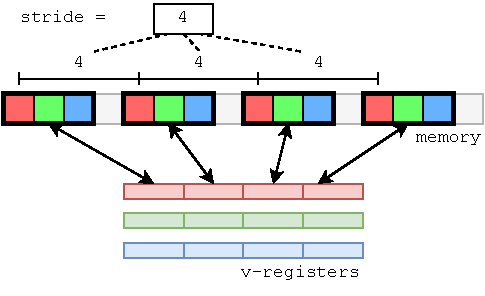
\includegraphics[width=\textwidth]{Figures/RVV_mem_strided_3seg.pdf}
        \caption{Example of a segmented strided access\\\code{EEW=8-bits}, \code{nf=3}, \code{stride=4},\code{EVL=4}}
        \label{fig:RVV_mem_strided_3seg}
    \end{subfigure}
    \caption{Segmented Unit/Strided Access Information}
\end{figure}

\noindent
This archetype moves active elements of \paramt{nf} vector register groups to/from contiguous segments of memory,
where the start of each segment is separated by \code{stride} bytes.

\begin{itemize}
    \item Unit-stride instructions tightly pack segments, i.e. \code{stride = \param{nf} * \param{eew} / 8}.
    \item Strided instructions read \code{stride} from register \code{rs2}.
    \begin{itemize}
        \item \code{stride} may be positive, negative, or zero.
    \end{itemize}
    % These two are described by the diagram
    % \item Each segment is \code{\param{nf} * \param{eew}} bits long, i.e. \paramt{nf} elements long.
    % \item Each element in the $i$-th segment maps to the $i$-th element of a vector register group.
    \item These instructions don't do anything if \code{vstart >= EVL}.
\end{itemize}

Strided accesses where \code{rs2} is register \code{x0} may perform fewer than \code{EVL} memory accesses.
Otherwise, even if \code{stride = 0}, implementations must appear to perform all accesses.

% ORDERING
\subsubsection*{Ordering}
There are no ordering guarantees, other than those required by precise vector traps (if used).

% EXCEPTION HANDLING
\subsubsection*{Exception Handling}
If any element within segment $i$ triggers a synchronous exception, \code{vstart} is set to $i$ and a precise or imprecise trap is triggered.
Load instructions may overwrite active segments past the segment index at which the trap is reported, but not past \code{EVL}.\cite[Section 7.7]{specification-RVV-v1.0}
Upon entering a trap, it is implementation-defined how much of the faulting segment's accesses are performed.

\subsection{Unit fault-only-first loads}\label{chap:bg:sec:rvv:fof}

\begin{figure}[h]
    \centering
    \begin{subtable}{\textwidth}
        \centering
        \begin{tabular}{lccc}
            \toprule
            Mnemonic & Data & Address & Masked \\
            \midrule
            \large\code{vlseg\param{<nf>}e\param{<eew>}ff.v} & \large\code{vd,} & \large\code{(rs1),} & \large\code{vm} \\
            \bottomrule
        \end{tabular}
        \caption{Instruction}
    \end{subtable}


    \begin{subtable}{\textwidth}
        \centering
        \begin{tabular}{ll}
                \toprule
                Masked? & \code{vm == 0} \\
                    \code{EEW} & \paramt{<eew>} \\
                    \code{EVL} & \code{vl} \\
                    \code{EMUL} &  \code{VLEN * \param{<eew>} / EVL} \\
                    \code{NFIELDS} & \paramt{<nf>} \\
                \bottomrule
            \end{tabular}
            \caption{Parameters}
    \end{subtable}

    \caption{Unit Fault-only-First Information}
    \label{tab:RVV_mem_fof}
\end{figure}


This archetype is equivalent to a unit load in all respects but exception handling.
If any access in segment 0 raises an exception\footnote{Segment 0 may be masked out, in which case this is impossible.}, \code{vl} is not modified and the trap is taken as usual.
If any access in any active segment $> 0$ raises an exception, the trap is not taken, \code{vl} is reduced to the index of the offending segment, and the instruction finishes.
If an asynchronous interrupt is encountered at any point, the trap is taken and \code{vstart} is set as usual.

This archetype is intended for \enquote{loops with data-dependent exit conditions}, and is commonly used for string operations.
The specification uses it in a \code{strcmp} example~(\cite[Section~A.9]{specification-RVV-v1.0}).

Similar to plain loads, if an exception is encountered the instruction is allowed to update segments past the offender (but not past the original \code{vl}).
If any synchronous exception or asynchronous interrupt occurs, regardless of the segment index, it is implementation-defined how much of the faulting segment's accesses are performed.

\pagebreak
%%%%%%%%%%%%%%%%%%%%%%%%%%%%%%%%%%%%%%%%%%
\subsection{Indexed accesses}\label{rvv:indexedmem}
\begin{figure}[h]
    \centering
    \begin{subtable}{\textwidth}
        \centering
        \begin{tabular}{lcccc}
            \toprule
        Mnemonic & Data & Address & Indices & Masked \\
        \midrule 
        \large\code{vl\param{<u|o>}xseg\param{<nf>}e\param{<eew>}.v} & \large\code{vd,} & \large\code{(rs1),} & \large\code{vs2,} & \large\code{vm} \\
        \bottomrule
        \end{tabular}
        \caption{Instruction}
    \end{subtable}
    \vspace{1em}
    
    \begin{subtable}[t]{0.5\textwidth}
        \centering
        \begin{tabular}[b]{ll}
    \toprule
        Masked? & \code{vm == 0} \\
    \midrule
        Element \code{EEW} & \code{vtype.SEW} \\
        Element \code{EMUL} & \code{vtype.LMUL} \\
        \midrule
        Ordered? & \paramt{<u|o>} \\
        Index Vector & \code{vs2} \\
        Index \code{EEW} & \paramt{<eew>} \\
        Index \code{EMUL} & \code{VLEN * \param{<eew>} / EVL} \\
        \midrule
        \code{NFIELDS} & \paramt{<nf>} \\
        \code{EVL} & \code{vl} \\
        \bottomrule
    \end{tabular}
    \caption{Parameters}
    \label{tab:RVV_mem_index}
    \end{subtable}\hfill
    \begin{subfigure}[t]{0.45\textwidth}
        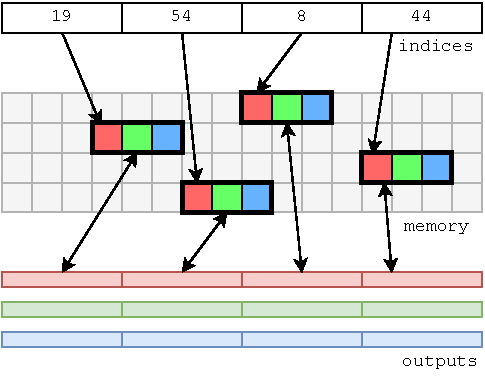
\includegraphics[width=\textwidth]{Figures/RVV_mem_index_3seg.pdf}
        \caption{Example of a segmented indexed access\\\code{EEW=8-bits}, \code{nf=3}}
        \label{fig:RVV_mem_index_3seg}
    \end{subfigure}
    \caption{Segmented Indexed Access Information}
\end{figure}

This archetype moves elements of \paramt{nf} vector register groups to/from contiguous segments of memory,
where each segment is offset by an index (in bytes) taken from another vector.

\begin{itemize}
\item The start of each segment is defined by \code{address + index\_vector[i]}.
\item These instructions don't do anything if \code{vstart >= EVL}.
\item Indexed segment loads may not overwrite the index vector\footnote{This allows restarting after raising an exception partway through a structure}.
\end{itemize}

% ORDERING
\subsubsection*{Ordering}
Accesses within each segment are not ordered relative to each other.
If the ordered variant of this instruction is used, then the segments must be accessed in order (i.e. 17, 53, 8, 44 for \cref{fig:RVV_mem_index_3seg}).
Otherwise, segment ordering is not guaranteed.


% EXCEPTION HANDLING
\subsubsection*{Exception Handling}
If any element within segment $i$ triggers a synchronous exception, \code{vstart} is set to $i$ and a precise or imprecise trap is triggered.
Load instructions may overwrite active segments past the segment index at which the trap is reported, but not past \code{EVL}\cite[Section 7.7]{specification-RVV-v1.0}.
Upon entering a trap, it is implementation-defined how much of the faulting segment's accesses are performed.

\pagebreak
\subsection{Unit whole-register accesses}

\begin{figure}[h]
    \centering

    \begin{subtable}[t]{0.5\textwidth}
        \centering
        \begin{tabular}{lcc}
            \toprule
            Mnemonic & Data & Address \\
            \midrule
            \large\code{vl\param{<nreg>}re\param{<eew>}.v} & \large\code{vd,} & \large\code{(rs1)} \\
            \bottomrule
        \end{tabular}
        \caption{Instruction}
    \end{subtable}\hfill
    \begin{subtable}[t]{0.5\textwidth}
        \centering
\begin{tabular}{ll}
\toprule
        Masked? & False \\
        Registers & \paramt{<nreg>} \\
        \code{EEW} & \paramt{<eew>} \\
        \code{EVL} & \code{NFIELDS * VLEN / EEW} \\
        \code{EMUL} & 1 \\
    \bottomrule
\end{tabular}
\caption{Parameters}
\end{subtable}
    \caption{Unit Whole Register Information}
    \label{tab:RVV_mem_wholereg}
\end{figure}

This archetype moves the contents of \paramt{nreg} vector registers to/from a contiguous range in memory.
Equivalent to a unit-stride access where \code{EVL} equals the total number of elements in \paramt{nreg} registers.
\begin{itemize}
    \item \code{nreg} must be a power of two.
    \item These instructions don't support segmented access.
    \item These instructions don't do anything if \code{vstart >= EVL}.
\end{itemize}

Ordering and exception handling are identical to unit-stride accesses (\cref{chap:bg:sec:rvv:unitstrideaccess}).

\subsection{Unit bytemask accesses}
\begin{figure}[h]
    \centering
    \begin{subtable}[t]{0.5\textwidth}
        \centering
        \begin{tabular}{lcc}
            \toprule
            Mnemonic & Data & Address \\
            \midrule
            \large\code{vlm.v} & \large\code{vd,} & \large\code{(rs1)} \\
            \bottomrule
        \end{tabular}
        \caption{Instruction}
    \end{subtable}\hfill
    \begin{subtable}[t]{0.5\textwidth}
        \centering
\begin{tabular}{ll}
    \toprule
        Masked? & False \\
        \code{EEW} & 8-bits \\
        \code{EVL} & \code{ceil(vl/8)} \\
        \code{EMUL} & 1 \\
    \bottomrule
\end{tabular}
\caption{Parameters}
\end{subtable}
    \caption{Unit Bytemask Information}
    \label{tab:RVV_mem_bytemask}
    % \end{subtable}\hfill
\end{figure}

This archetype moves the contents of a mask register to/from a contiguous range of memory.
It transfers at least \code{vl} bits, one bit for each element that could be used in subsequent vector instructions.
This will always fit in a single vector register (see \cref{chap:bg:subsec:rvvmasking}), hence \code{EMUL = 1} in all cases.
\begin{itemize}
    \item These instructions operate as if the tail-agnostic setting of \code{vtype} is true.
    \item These instructions don't support segmented access.
    \item These instructions don't do anything if \code{vstart >= EVL}.
\end{itemize}
Ordering and exception handling are identical to unit-stride accesses (\cref{chap:bg:sec:rvv:unitstrideaccess}).
\pagebreak
\section{Previous RVV implementations\label{chap:bg:rvvend}}
Even before v1.0 of the RVV specification was released, multiple implementations were released in academia and industry.
These implementations showcase the diversity allowed by a scalable model: \citeauthor{johnsMinimalRISCVVector2020} integrated a minimal vector processor into a scalar pipeline meant for microcontrollers (\code{VLEN=32}) \cite{johnsMinimalRISCVVector2020}, \citeauthor{dimascioOnBoardDecisionMaking2021} employed a RVV implementation for deep learning in space\cite{dimascioOnBoardDecisionMaking2021}, and AndesCode, SiFive, and Alibaba have released cores with \code{VLEN}s up to 512\cite{AndesCoreNX27VProcessor}\cite{SiFiveIntelligenceX280}\cite{chenXuantie910CommercialMultiCore2020}.
Other academic examples include Ara\cite{cavalcanteAra1GHzScalable2020}, Arrow\cite{assirArrowRISCVVector2021}, RISC-$\text{V}^2$\cite{patsidisRISCV2ScalableRISCV2020}, and Vicuna\cite{platzerVicunaTimingPredictableRISCV2021}, which all decouple the vector processing from the scalar pipeline\footnote{These implementations are not examined further as they do not go into detail on their load/store implementations.}.
% \todomark{Planned to do a survey of existing implementations here - might be too many words?}

This is only going to continue: multiple implementations were just recently presented at RISC-V Week in Paris (May 2022).
Vitruvius\cite{minerviniVitruviusAreaEfficientRISCV2022} uses extremely long vectors \code{VLEN=256*64=16384}, is implemented as a decoupled processor, and is the first RISC-V processor to support the Open Vector Interface (OVI)\footnote{\gitrepo{semidynamics/OpenVectorInterface}{https://github.com/semidynamics/OpenVectorInterface}} for communicating with the scalar core.
VecProM\cite{mahaleRISCVVPUVery2021} splits its approach into two, where vectors beyond a certain length are strip-mined and processed in hardware using a scratch memory, using OVI to connect multiple heterogeneous vector processors to a scalar core.
Both were produced from the Barcelona Supercomputing Center under the European Processor Initiative.

% \todomark{This is only going to continue: an implementation was presented at RISC-V week(cite)}
% Vitruvius: 256 * 64-bit elements
% Decoupled processor
% Uses OVI to communicate with scalar cores
\pagebreak
\section{CHERI}\label{chap:bg:sec:cheri}
% Concept of a capability
In CHERI, addresses/pointers are replaced with capabilities: unforgeable tokens that provide \emph{specific kinds of access} to an \emph{address} within a \emph{range of memory}.
The above statement is enough to understand what capabilities contain\footnote{This is a slight simplification. For the purposes of vector memory accesses the \emph{otype} of a capability can be ignored, as any type other than \code{UNSEALED} cannot be dereferenced anyway.}:
\begin{itemize}
    \item Permission bits, to restrict access
    \item The \emph{cursor}, i.e. the address it currently points to
    \item The \emph{bounds}, i.e. the range of addresses this capability could point to
\end{itemize}
A great deal of work has gone into compressing capabilities down into a reasonable size (see \cite{woodruffCHERIConcentratePractical2019}, \todomark{add diagram from TR-941?}), and using the magic of floating-point all of this data has been reduced to just 2x the architectural register size.
For example, on 64-bit RISC-V a standard capability is 128-bits long.
The rest of this dissertation assumes capabilities are 128-bits long for simplicity.

A CHERI implementation has to enforce three security properties about its capabilities\todocite[Section 1.2.1]{TR-951}:
\begin{itemize}
    \item Provenance - Capabilities must always be derived from valid manipulations of other capabilities.
    \item Integrity - Corrupted capabilities cannot be dereferenced.
    \item Monotonicity - Capabilities cannot increase their rights.
\end{itemize}

Integrity is enforced by tagging registers and memory.
Every 128-bit register and aligned 128-bit region of memory has an associated tag bit, which denotes if its data encodes a valid capability\footnote{This has the side-effect that capabilities must be 128-bit aligned in memory.}.
If any non-capability data is written to any part of the region the tag bit is zeroed out.
Instructions that perform memory accesses can only do so if the provided capability has a valid tag bit.
As above, significant work has gone into the implementation to reduce the DRAM overhead of this method (see \cite{joannouEfficientTaggedMemory2017} for an example).

Provenance and Monotonicity are enforced by all instructions that manipulate capabilities.
If an implementation detects a violation of either property, it will zero out the tag bit and rely on Integrity enforcement to ensure it is not dereferenced.
Some CHERI-enabled architectures, such as CHERI-RISC-V, also raise a synchronous exception when this occurs.

\subsection{CHERI-RISC-V ISA}
The Cambridge Computer Lab's TR-951 report\todocite{TR-951} describes the latest version of the CHERI architecture (CHERI ISAv8) and proposes applications to MIPS, x86-64, and RISC-V.
CHERI-RISC-V is a mostly straightforward set of additions to basic RISC-V ISAs.
It adds thirty-two general-purpose capability registers, thirty-two Special Capability Registers (SCRs), and many new instructions.

The new general-purpose capability registers are each of size \code{CLEN = 2 * XLEN} plus a tag bit.
These registers store compressed capabilities.
While there is always a logical distinction between the pre-existing \emph{integer} registers \code{x0-x31} and the \emph{capability} registers \code{cx0-cx31}, the architecture may store them in a Split or Merged register file.
A Split register file stores the integer registers separately from capability registers, so programs can manipulate them independently.
A Merged register file stores thirty-two registers of length \code{CLEN}, using the full width for the capability registers, and aliases the integer registers to the bottom \code{XLEN} bits.
Under a merged register file, writing to an integer register makes the capability counterpart invalid, so programs have to be more careful with register usage.

\todomark{diagram for split/merged register file?}

Many of the new SCRs are intended to support the privileged ISA extensions for e.g. hypervisors or operating systems.
The emulator doesn't use these, so their SCRs are not listed here, but there are two highly relevant SCRs for all modes: the Program Counter Capability and the Default Data Capability.

The PCC replaces the program counter and adds more metadata, ensuring instruction fetches have the same security properties as normal loads and stores.
The DDC is used to sandbox integer addressing modes.
CHERI-RISC-V includes new instructions which use integer addressing, and allows legacy (i.e. integer addressed) code to function on CHERI systems without recompiling for CHERI-RISC-V.
These instructions all use integer addresses relative to the DDC, and the DDC controls the permissions those instructions have.

\subsection{Instruction changes}
TR-951\todocite[Chapter 8]{TR-951} specifies a suite of new instructions, as well as a set of modifications to pre-existing instructions.
Many of the new instructions are unrelated to pre-existing instructions, and implement capability-specific operations like accessing fields of capability registers.
The most relevant new instructions for our case are the various loads/stores.

CHERI-RISC-V adds new instructions for loading integer and capability data, either via capabilities or using integer addressing through the DDC (\cref{tab:new_cheri_instrs}).
These instructions are slightly more limited than the pre-existing counterparts, because they do not support immediate offsets. \todomark{is there rationale for that documented somewhere?}
To maintain compatibility with legacy programs that haven't been compiled for CHERI-RISC-V, the behaviour of basic RISC-V load/store opcodes changes to either use capabilities as memory references or use integer addressing via the DDC, depending on the encoding mode.

\begin{table}[h]
    \centering
    \begin{tabular}{lccl}
    \toprule
        Name & Direction & Data type & Address calculation \\
        \midrule
        L[BHWD][U].CAP & Load & Integer & via capability register \\
        L[BHWD][U].DDC & Load & Integer & via DDC \\
        LC.CAP & Load & Capability & via capability register \\
        LC.DDC & Load & Capability & via DDC \\ 
        S[BHWD].CAP & Store & Integer & via capability register \\
        S[BHWD].DDC & Store & Integer & via DDC \\
        SC.CAP & Store & Capability & via capability register \\
        SC.DDC & Store & Capability & via DDC \\ 
    \bottomrule
    \end{tabular}
    \caption{New CHERI load/store instructions}
    \label{tab:new_cheri_instrs}
\end{table}
\begin{table}[h]
    \centering
    \begin{tabular}{lccc}
    \toprule
        Name & Direction & Data type & \multicolumn{1}{c}{Address calculation} \\
        &&& (Capability/Integer mode) \\
        \midrule
        {[C]}LC\parnote{Replaces RV128 LQ} & Load & Capability & via capability/DDC \\
        {[C]}SC\parnote{Replaces RV128 SQ} & Store & Capability & via capability/DDC \\
        \midrule
        L[BWHD][U] & Load & Integer & via capability/DDC \\
        S[BWHD] & Store & Integer & via capability/DDC \\
        FL[WDQ] & Load & Float & via capability/DDC \\
        FS[WDQ] & Store & Float & via capability/DDC \\
        LR & Load & Integer & via capability/DDC \\
        SC & Store & Integer & via capability/DDC \\
        AMO\parnote{All atomic memory operations} & - & Integer & via capability/DDC \\
    \bottomrule
    \end{tabular}
    \parnotes
    \caption{Preexisting RISC-V load/store instructions modified by CHERI-RISC-V}
    \label{tab:legacy_cheri_instrs}
\end{table}

\subsection{Capability and Integer encoding mode\label{chap:bg:subsec:cheriencodingmode}}
CHERI-RISC-V specifies two encoding modes, selected using a flag in the PCC \code{flags} field.
\emph{Capability mode} modifies the behaviour of pre-existing instructions to take address operands as capabilities.
This makes the basic load/store instruction behaviour exactly equivalent to newly introduced counterparts: e.g. \code{L[BWHD][U] == L[BWHD][U].CAP}.
The DDC may still be used in this mode via the new instructions e.g. \code{S[BWHD].DDC}.

\emph{Integer mode} seeks to emulate a standard CHERI-less RISC-V architecture as much as possible.
All pre-existing RISC-V memory access instructions take address operands as integers, which are dereferenced relative to the DDC\footnote{Of course, the DDC must be valid when it is used in this mode, and all bounds checks etc. must still pass.}.
This makes the basic load/store instruction behaviour exactly equivalent to newly introduced counterparts: e.g. \code{L[BWHD][U] == L[BWHD][U].DDC}.
The new instructions may still be used to dereference and inspect capability registers, but all other instructions access registers in an integer context i.e. ignoring the upper bits and tag from merged register files.

\subsection{Pure-capability and Hybrid compilation modes}
CHERI's de facto compiler, CHERI-Clang\todocite{}, supports two ways to compile CHERI-RISC-V which map to the different encoding modes.

\emph{Pure-capability} mode treats all pointers as capabilities, and emits pre-existing RISC-V instructions that expect to be run in capability mode\footnote{This wasn't derived from documentation, but instead from manual inspection of emitted code.}.

\emph{Hybrid} mode treats pointers as integer addresses, dereferenced relative to the DDC, unless they are annotated with \code{\_\_capability}.
This mode allows programs to be gradually ported to CHERI, \todomark{which is important in ways I am too tired to express}
This mode emits pre-existing RISC-V instructions that take integer operands, and uses capabilities through the new instructions.
All capabilities in hybrid mode are created manually by the program by copying and shrinking the DDC.

\subsection{Capability relocations\label{chap:bg:subsec:cherirelocs}}
\todomark{Summarizes TR-494 Section 4.4, Appx C}
Binary applications compiled in pure-capability mode require some ``global'' capabilities to exist at startup, e.g. the capability which points to the \code{main()} function.
It would be a security risk to synthesize these capabilities from thin air, or to allow the binary file itself to contain tag bits.

Instead, CHERI ELF binaries contain a set of requested ``relocations'' (the \code{\_\_cap\_relocs} section) which instruct the runtime environment to create capabilities with specific permissions and bounds in specific places.
This process uses the normal CHERI capability instructions, so any invalid requests will cause a program crash, maintaining security.
Further complexity is introduced with dynamic linking, and in the future these relocations may change format, both described in \todocite{TR-494}, but the above description is sufficient to understand the rest of this paper.

% \subsection{Instruction reference}
% \todomark{TR-951 contains a complete reference of all added instructions in section blah, and notes legacy instructions modified by capability mode in section blah. Reproduce short list? Do so in appendix?}

\end{document}